\section{Results for two-dimensional heat equation}
\subsection{The case of constant diffusion coefficient}
In the previous sections we have found that the CG algorithm are much more efficient than the direct methods such as LU decomposition, so all the simulation for the two-dimentional equation have been done using CG method.
\\
\begin{figure}[ht]\centering
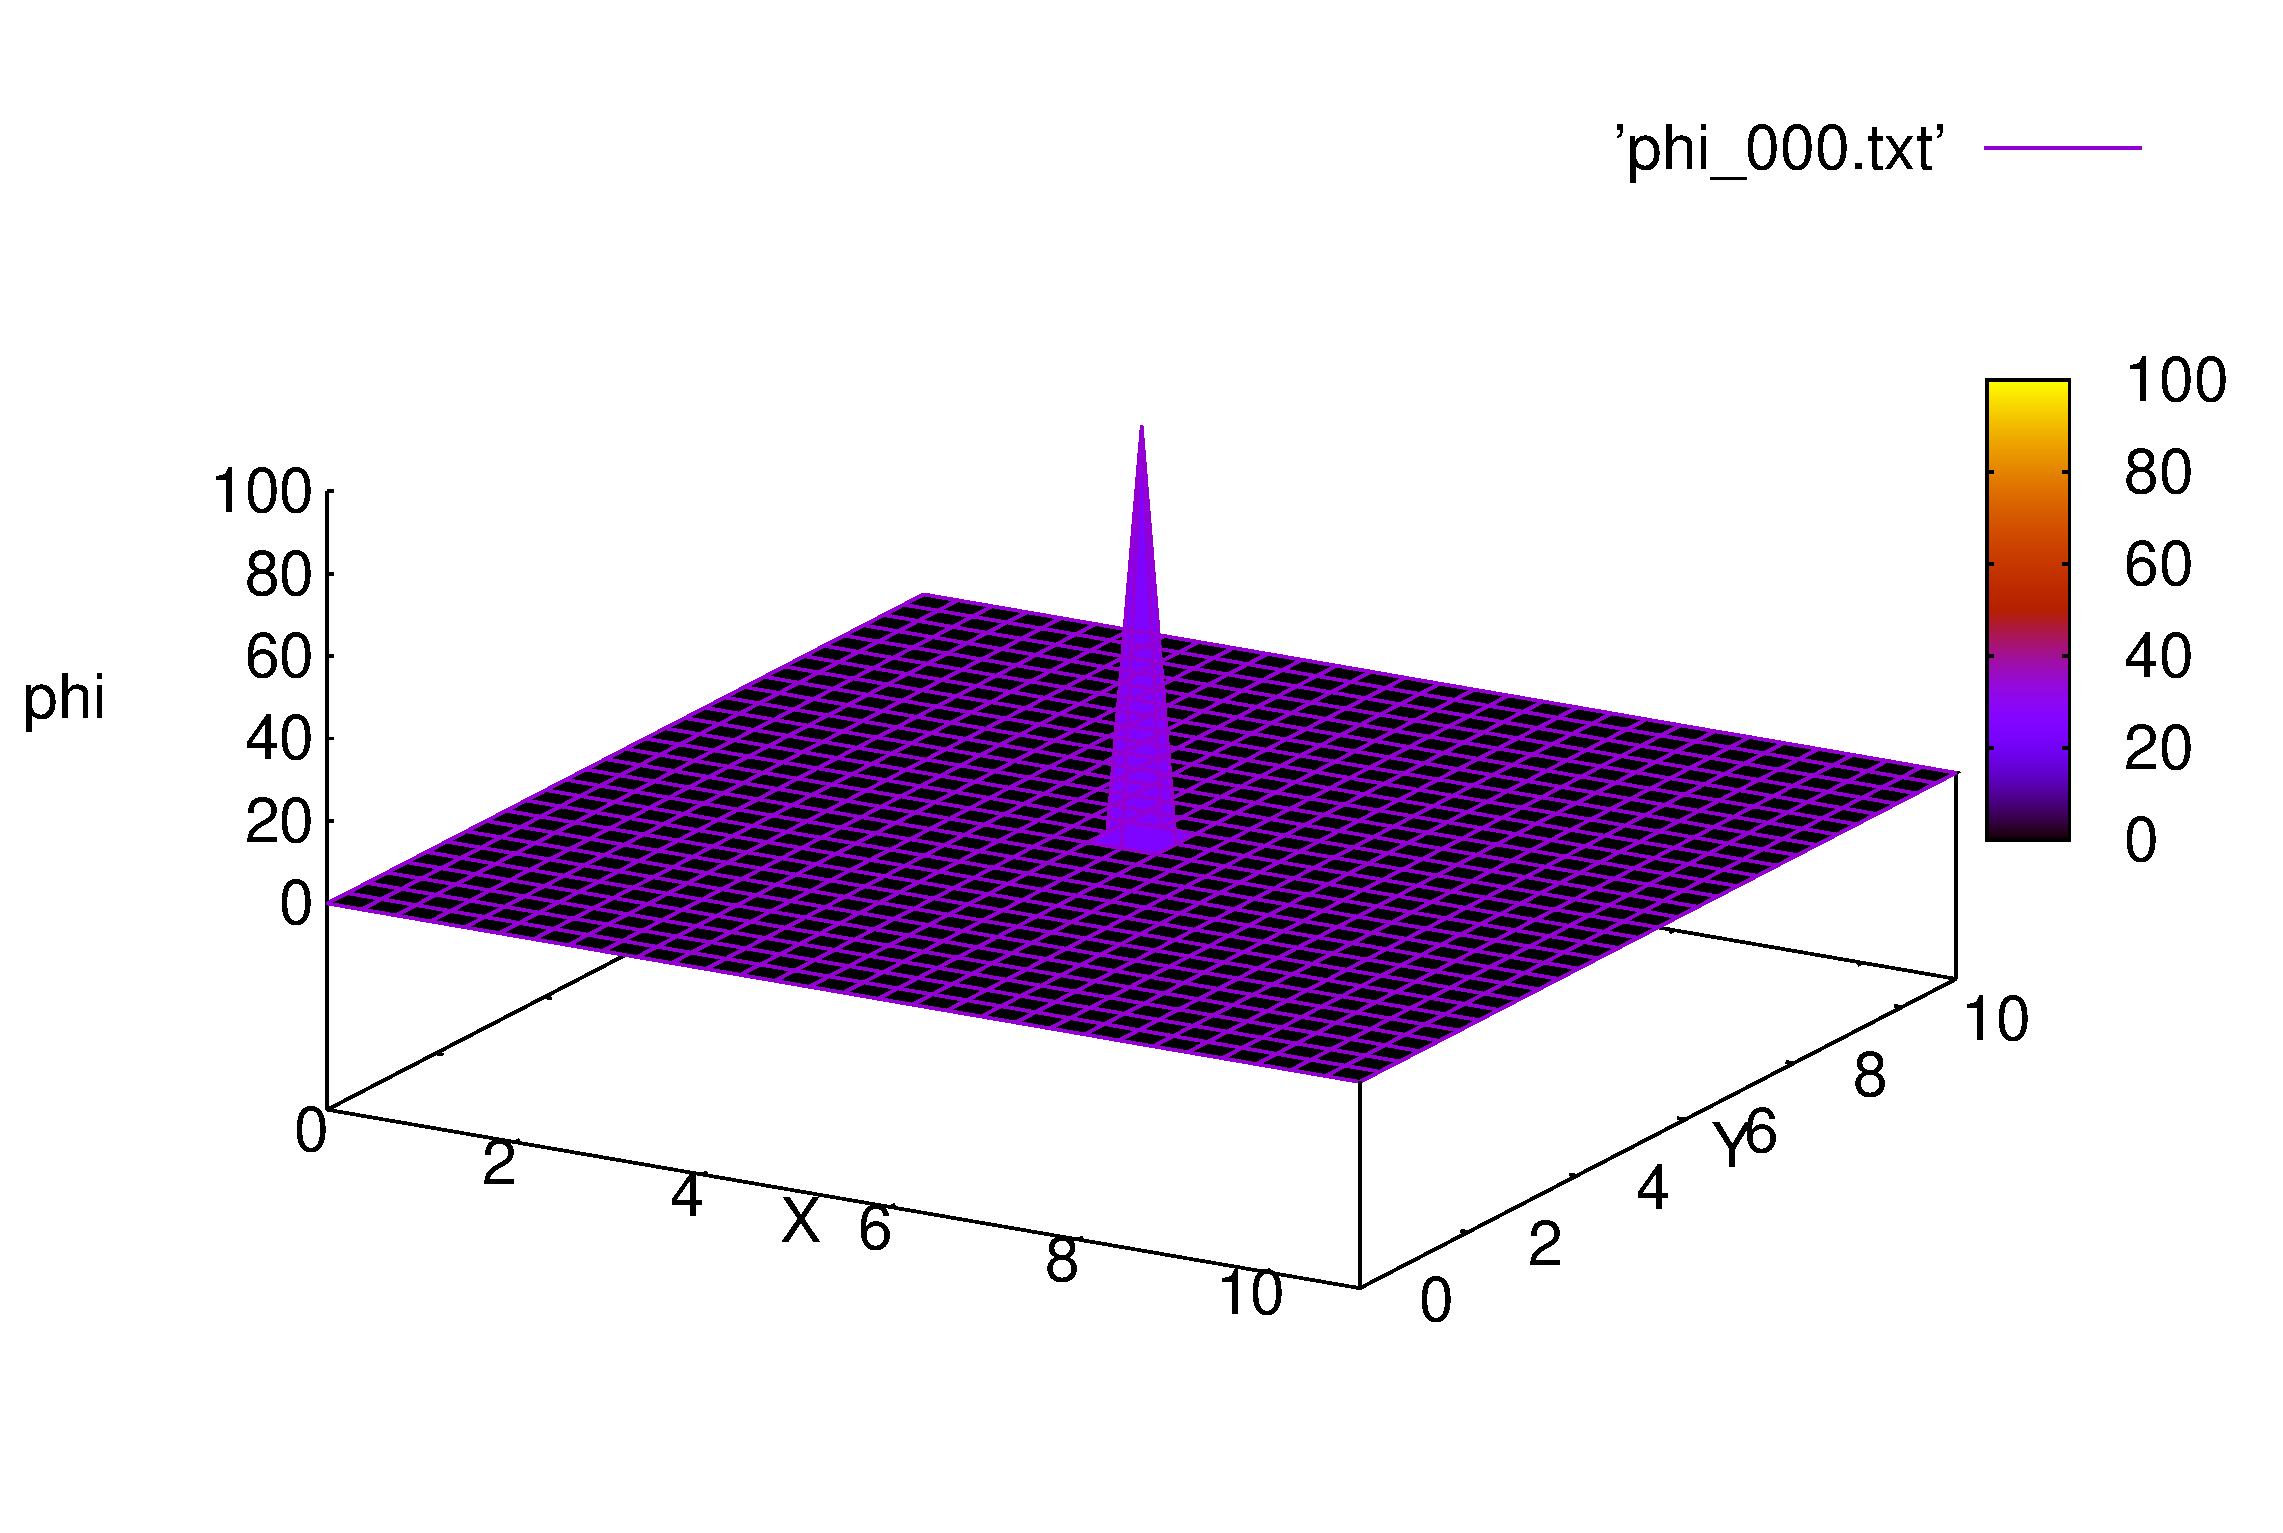
\includegraphics[width=\linewidth]{2DSimplefig/00}
\caption{initial condition for the 2D heat problem}
\label{fig:2d-initial_condition}
\end{figure}


%For the next step you will get figure \ref{fig:2d-1dt}.

%\begin{figure}[ht]\centering
%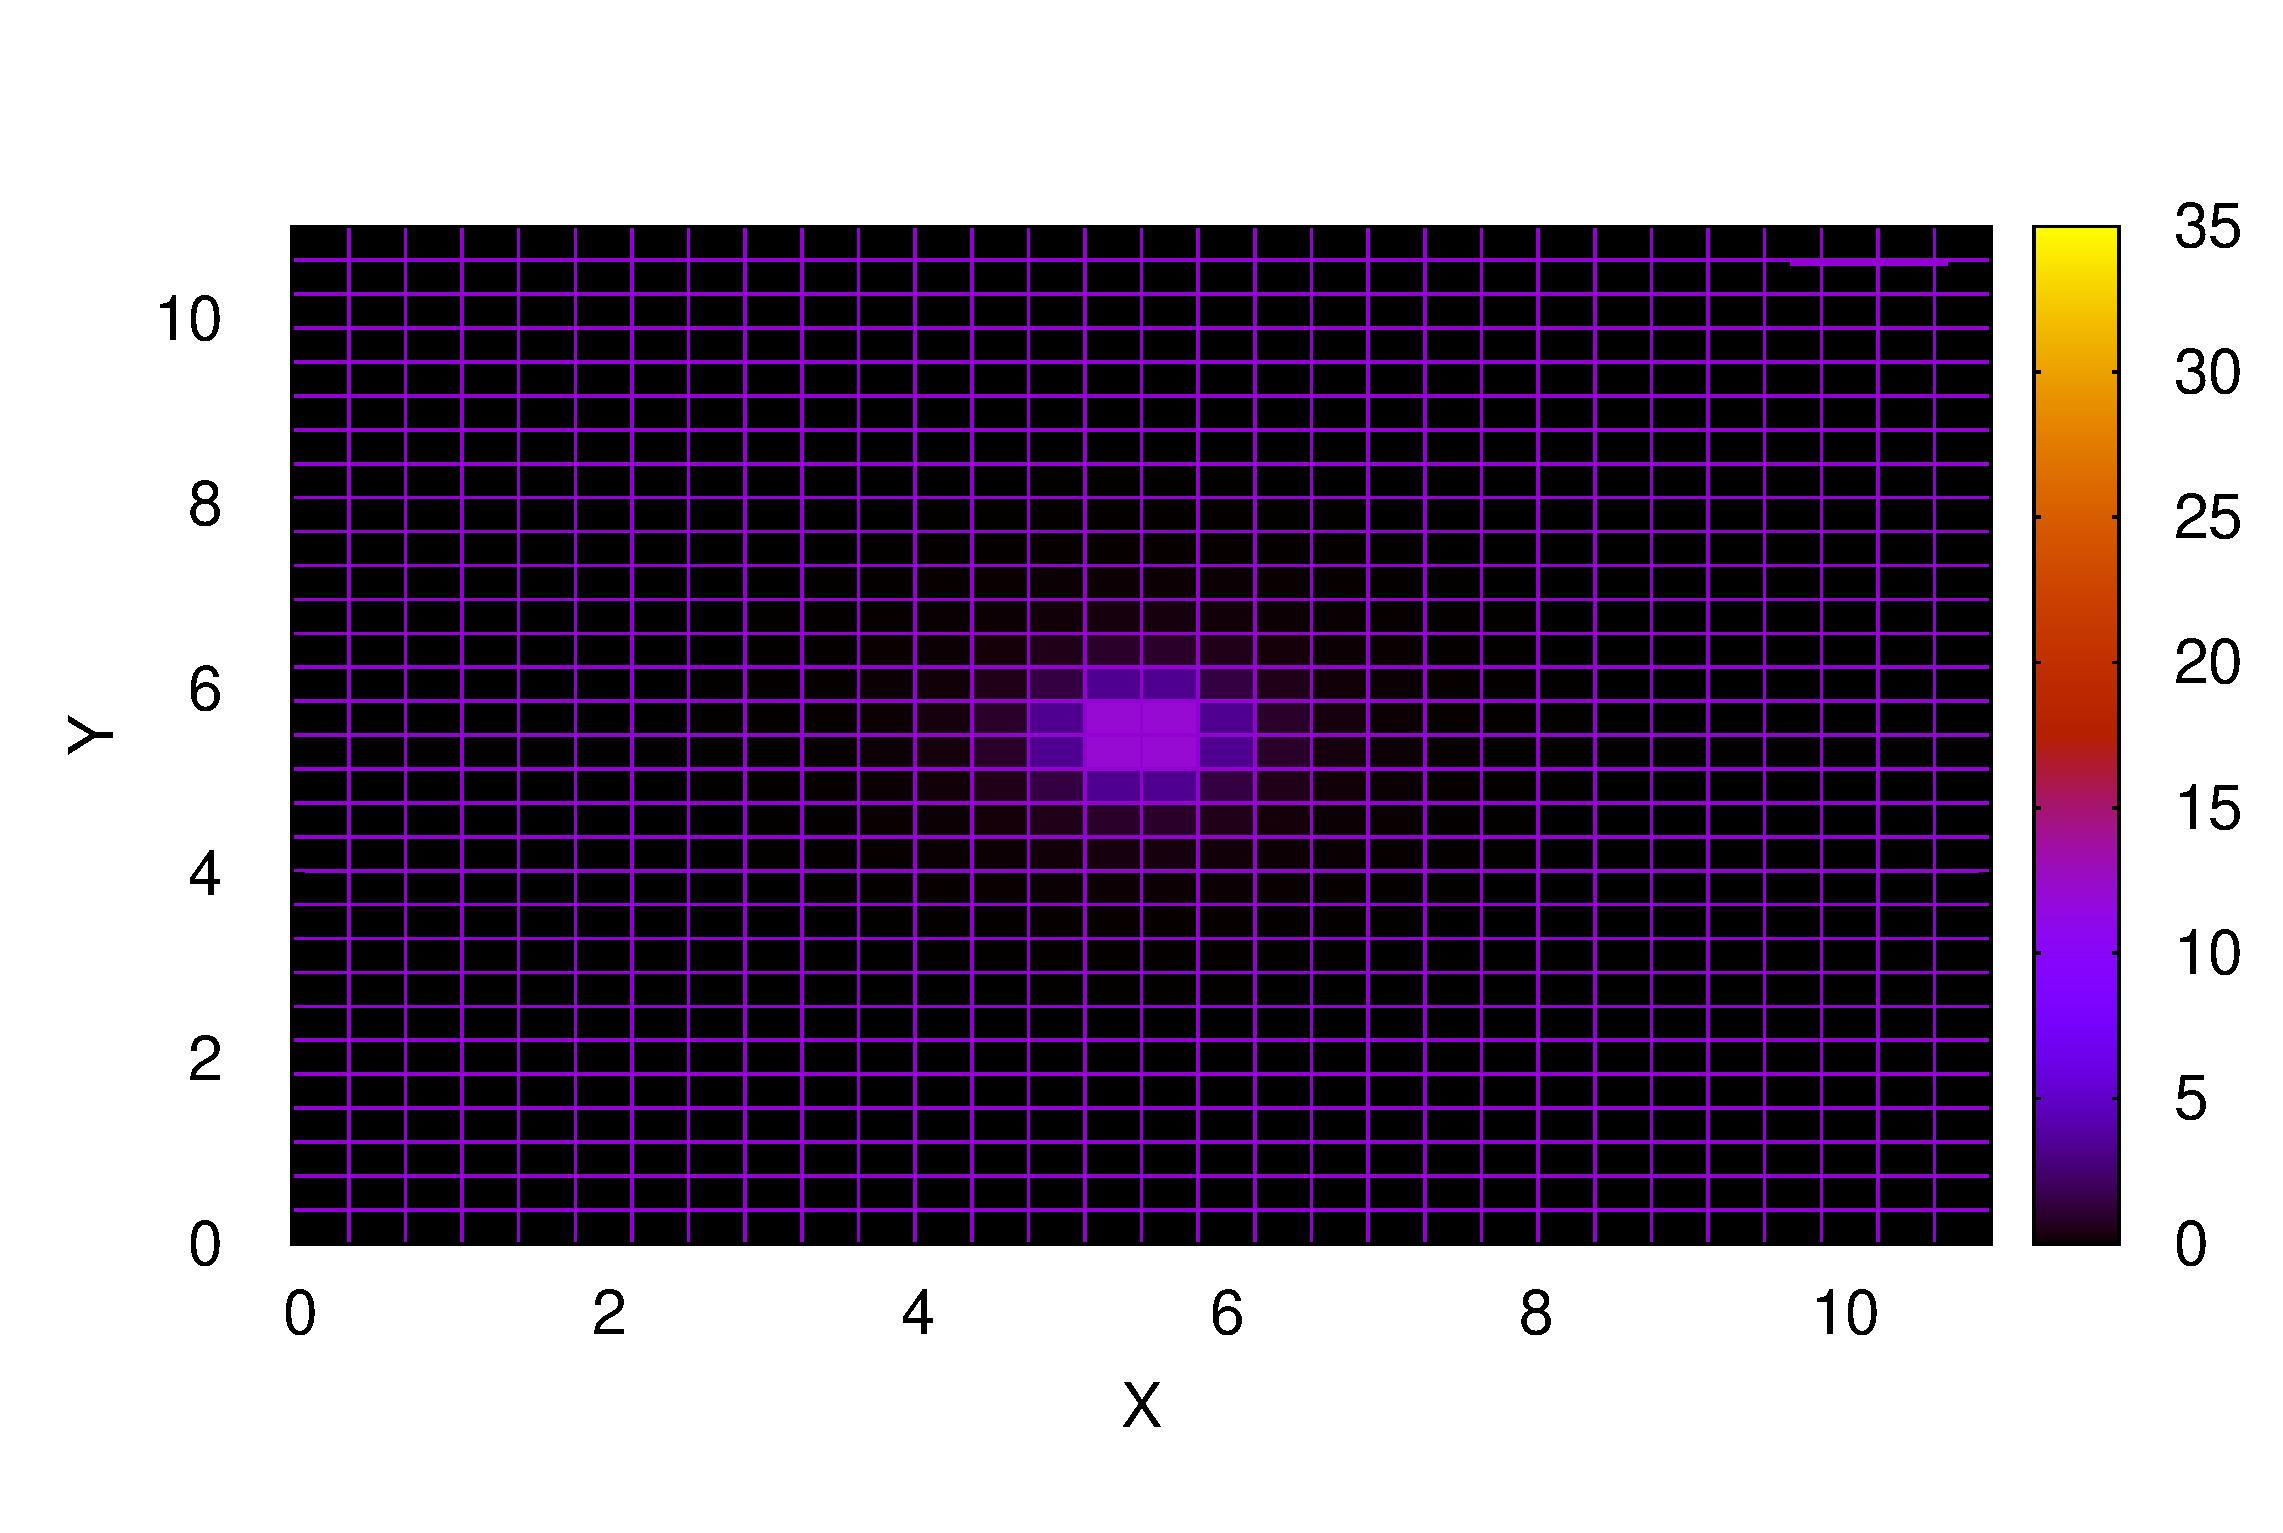
\includegraphics[width=\linewidth]{2DSimplefig/01_map}
%\caption{First step for the 2D heat problem}
%\label{fig:2d-1dt}
%\end{figure}

After 10 steps we will have figure \ref{fig:2d-10dt}. There is also an animation accessible at: \\
  \texttt{http://www.github.com/}. \\


\begin{figure}
     \centering
     \begin{subfigure}[b]{0.5\textwidth}
         \centering
         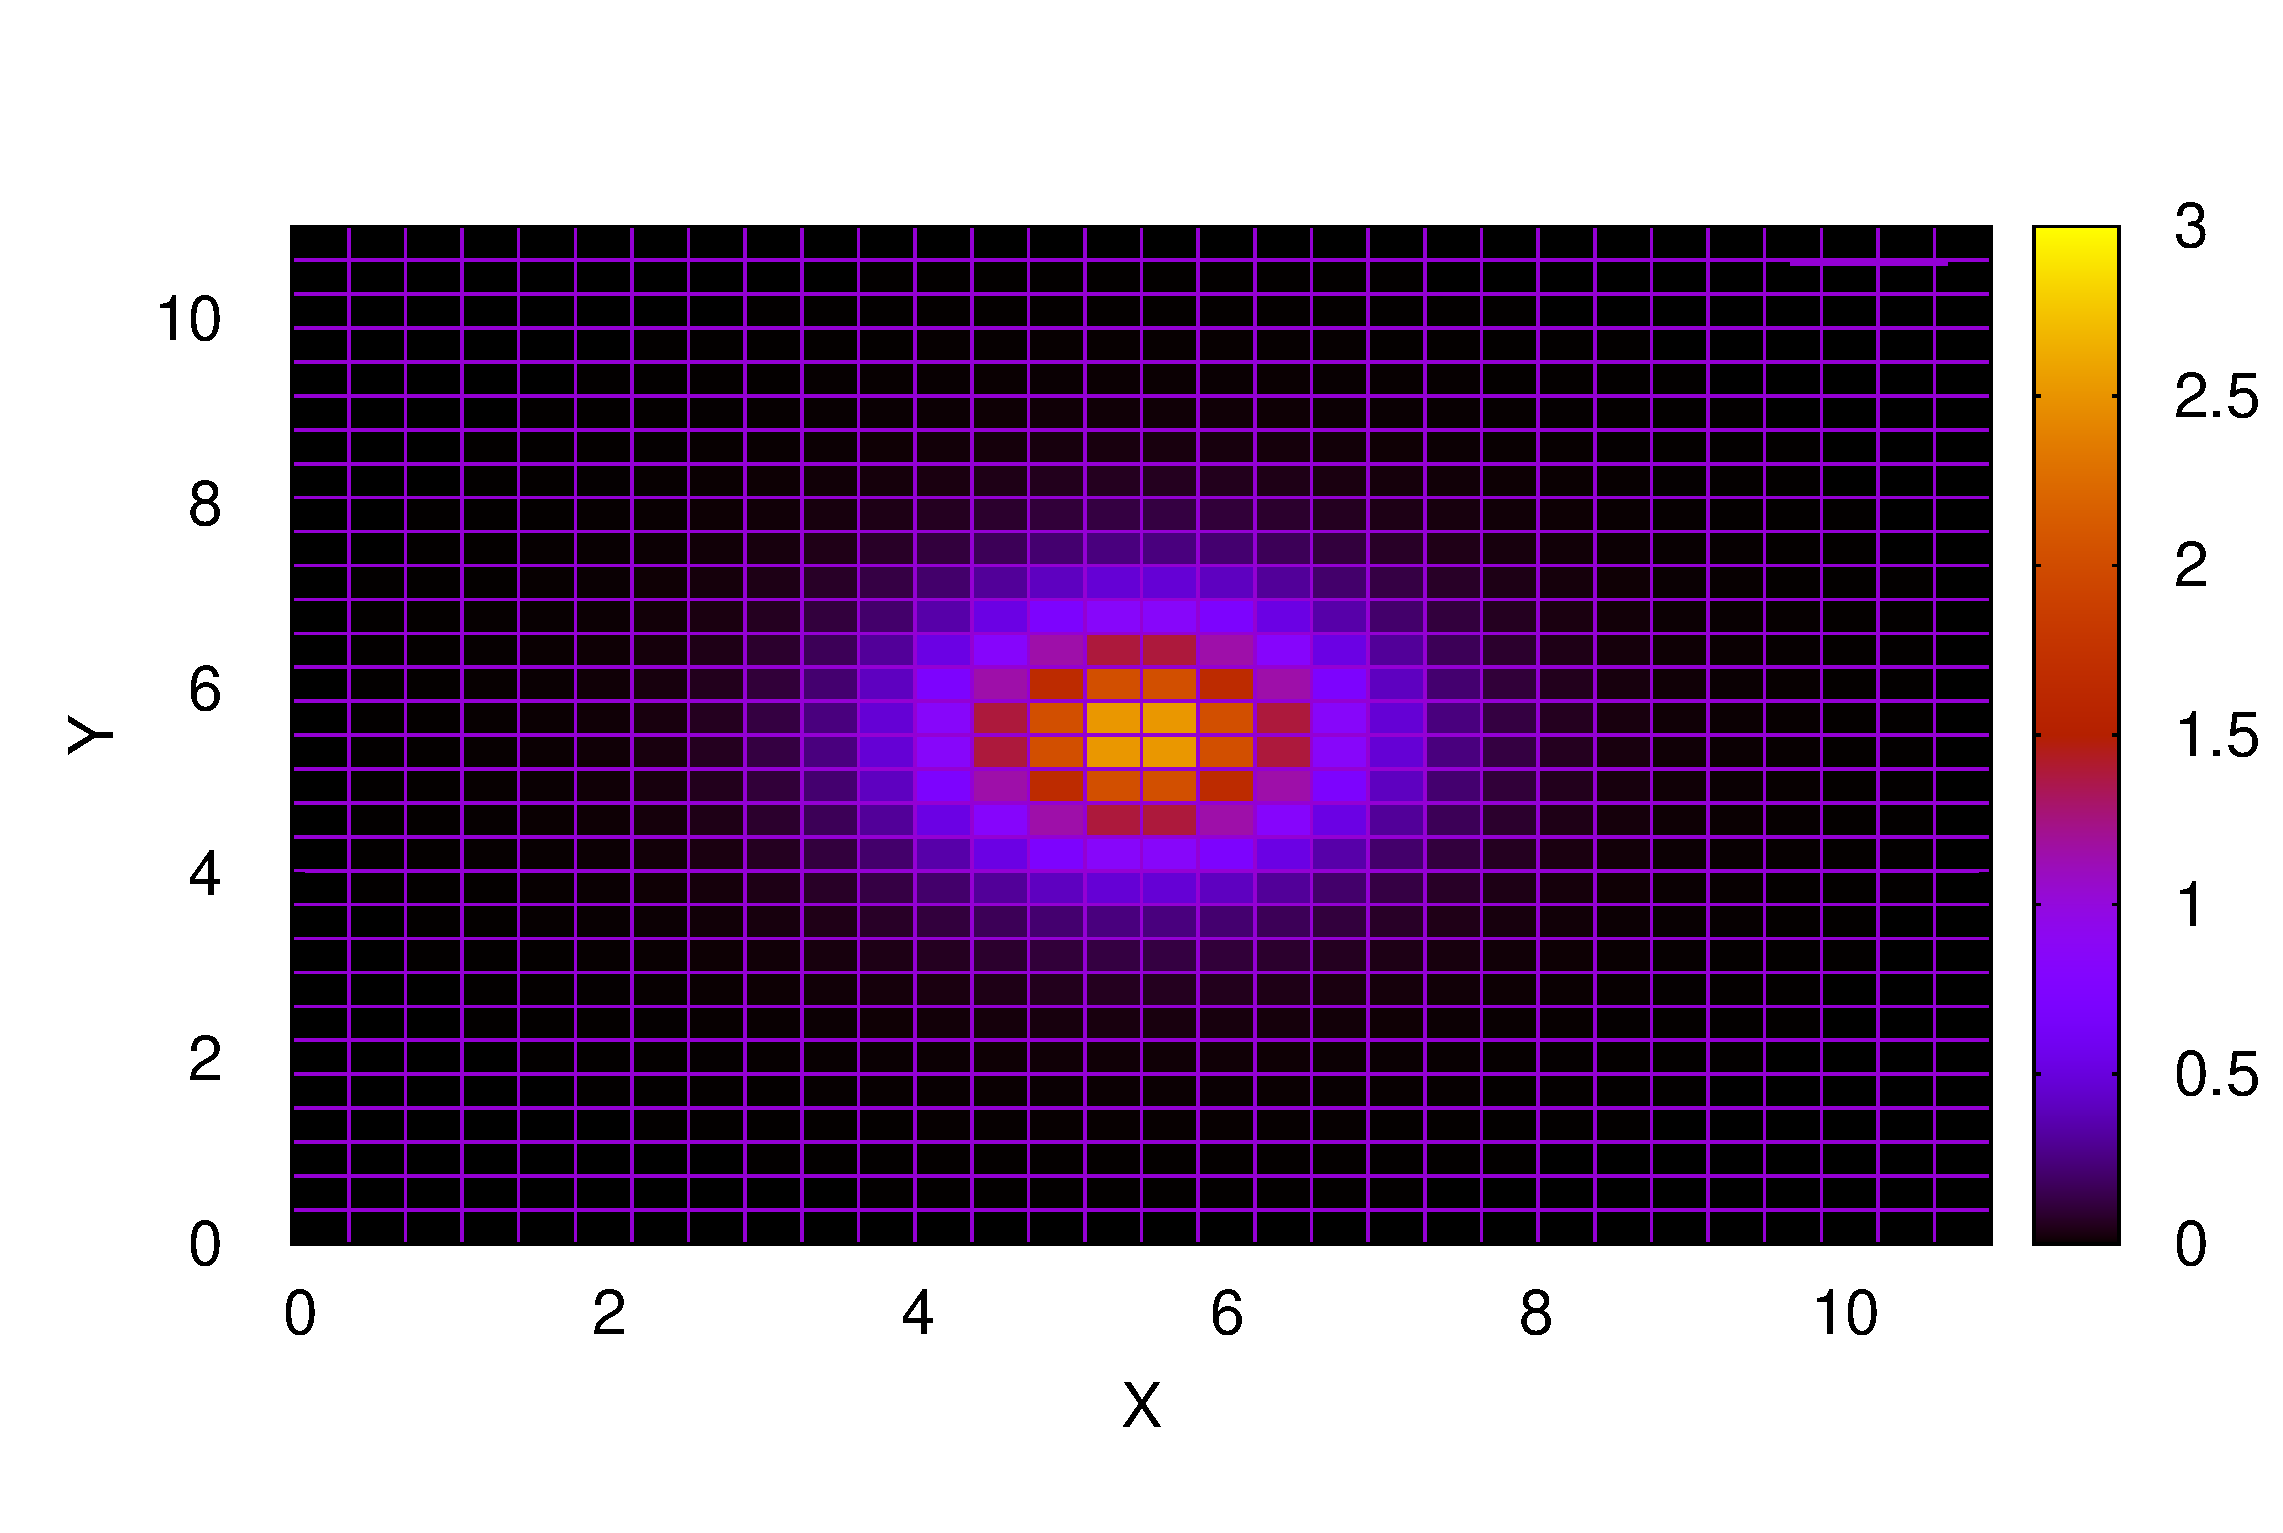
\includegraphics[width=\textwidth]{2DSimplefig/05_map}
		\caption{the heat distribution map after 5 timesteps for the 2D heat problem}
		\label{fig:2d-5dt}
     \end{subfigure}
     \hfill
	\centering
     \begin{subfigure}[b]{0.5\textwidth}
         \centering
         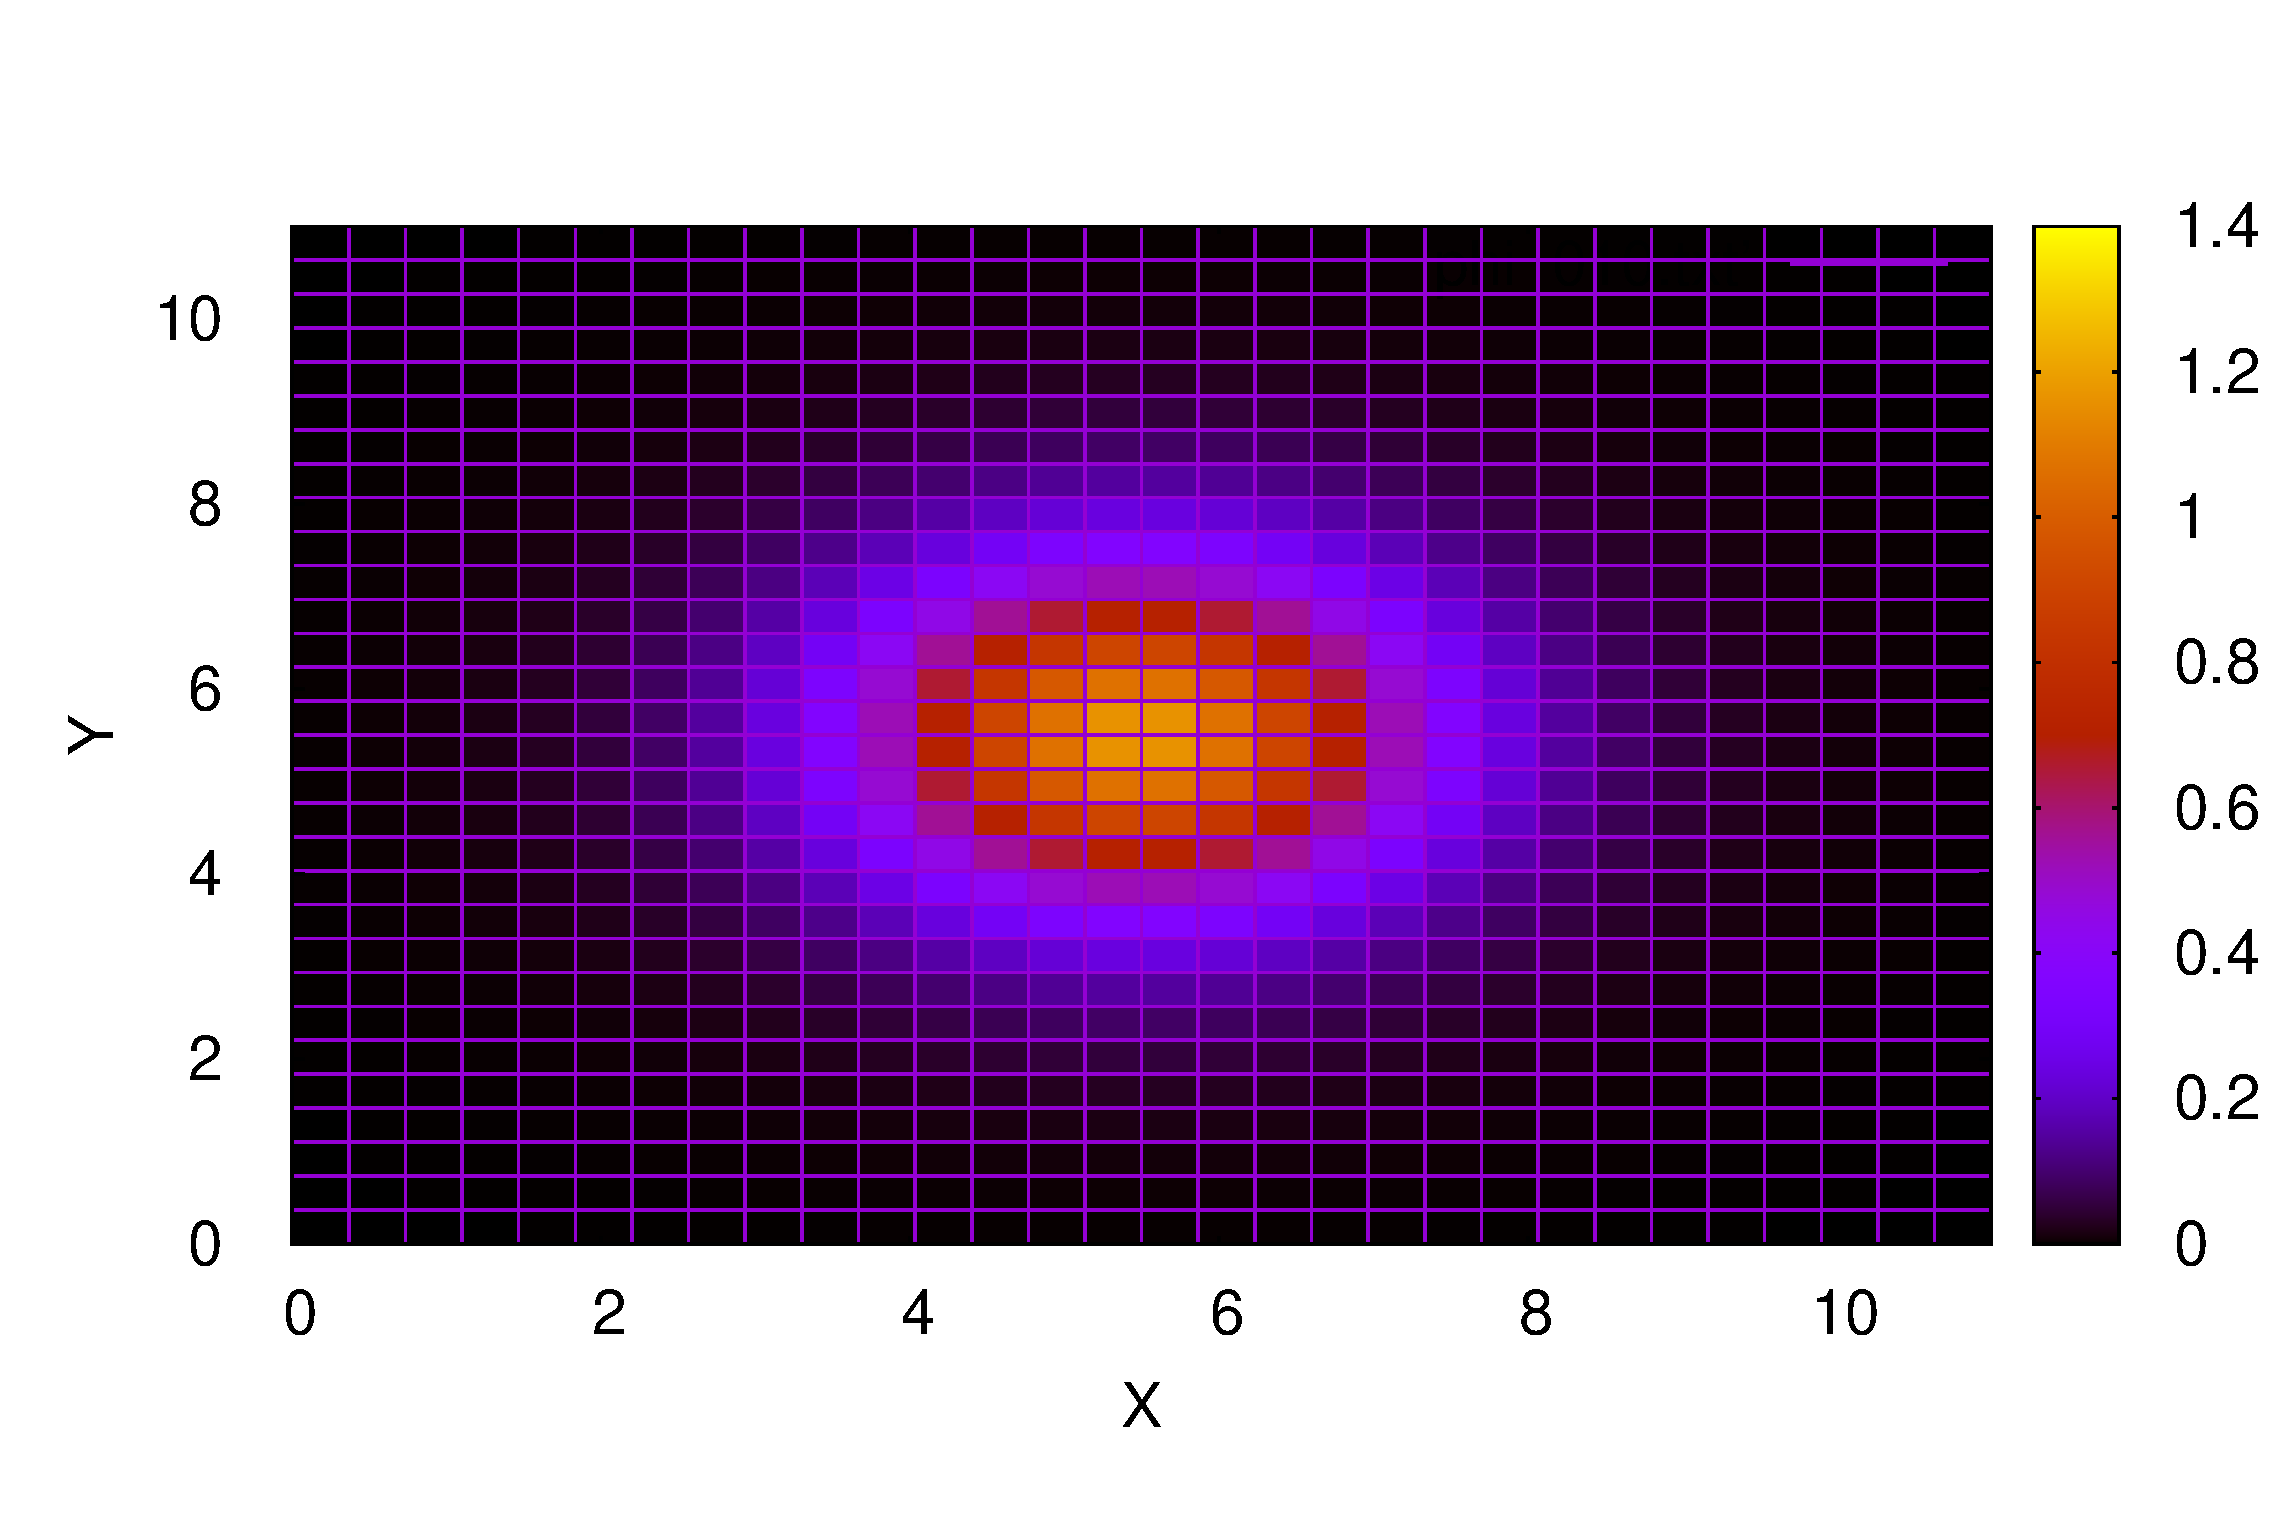
\includegraphics[width=\textwidth]{2DSimplefig/10_map}
		\caption{the heat distribution map after 10 timesteps for the 2D heat problem}
		\label{fig:2d-10dt}
     \end{subfigure}
     \hfill     
        \caption{solving two-dimensional heat equation using CG method.}
        \label{fig:2d-CG}
\end{figure}



In this case (constant diffusion coefficient), it is clear that the diffusion process is symmetric.
 \\

\subsection{The case of random diffusion coefficient}
The initial conditions of this case is the same as the initial condition for the constant diffusion coefficient (figure \ref{fig:2d-initial_condition}). 
\\

\begin{figure}
     \centering
     \begin{subfigure}[b]{0.45\textwidth}
         \centering
         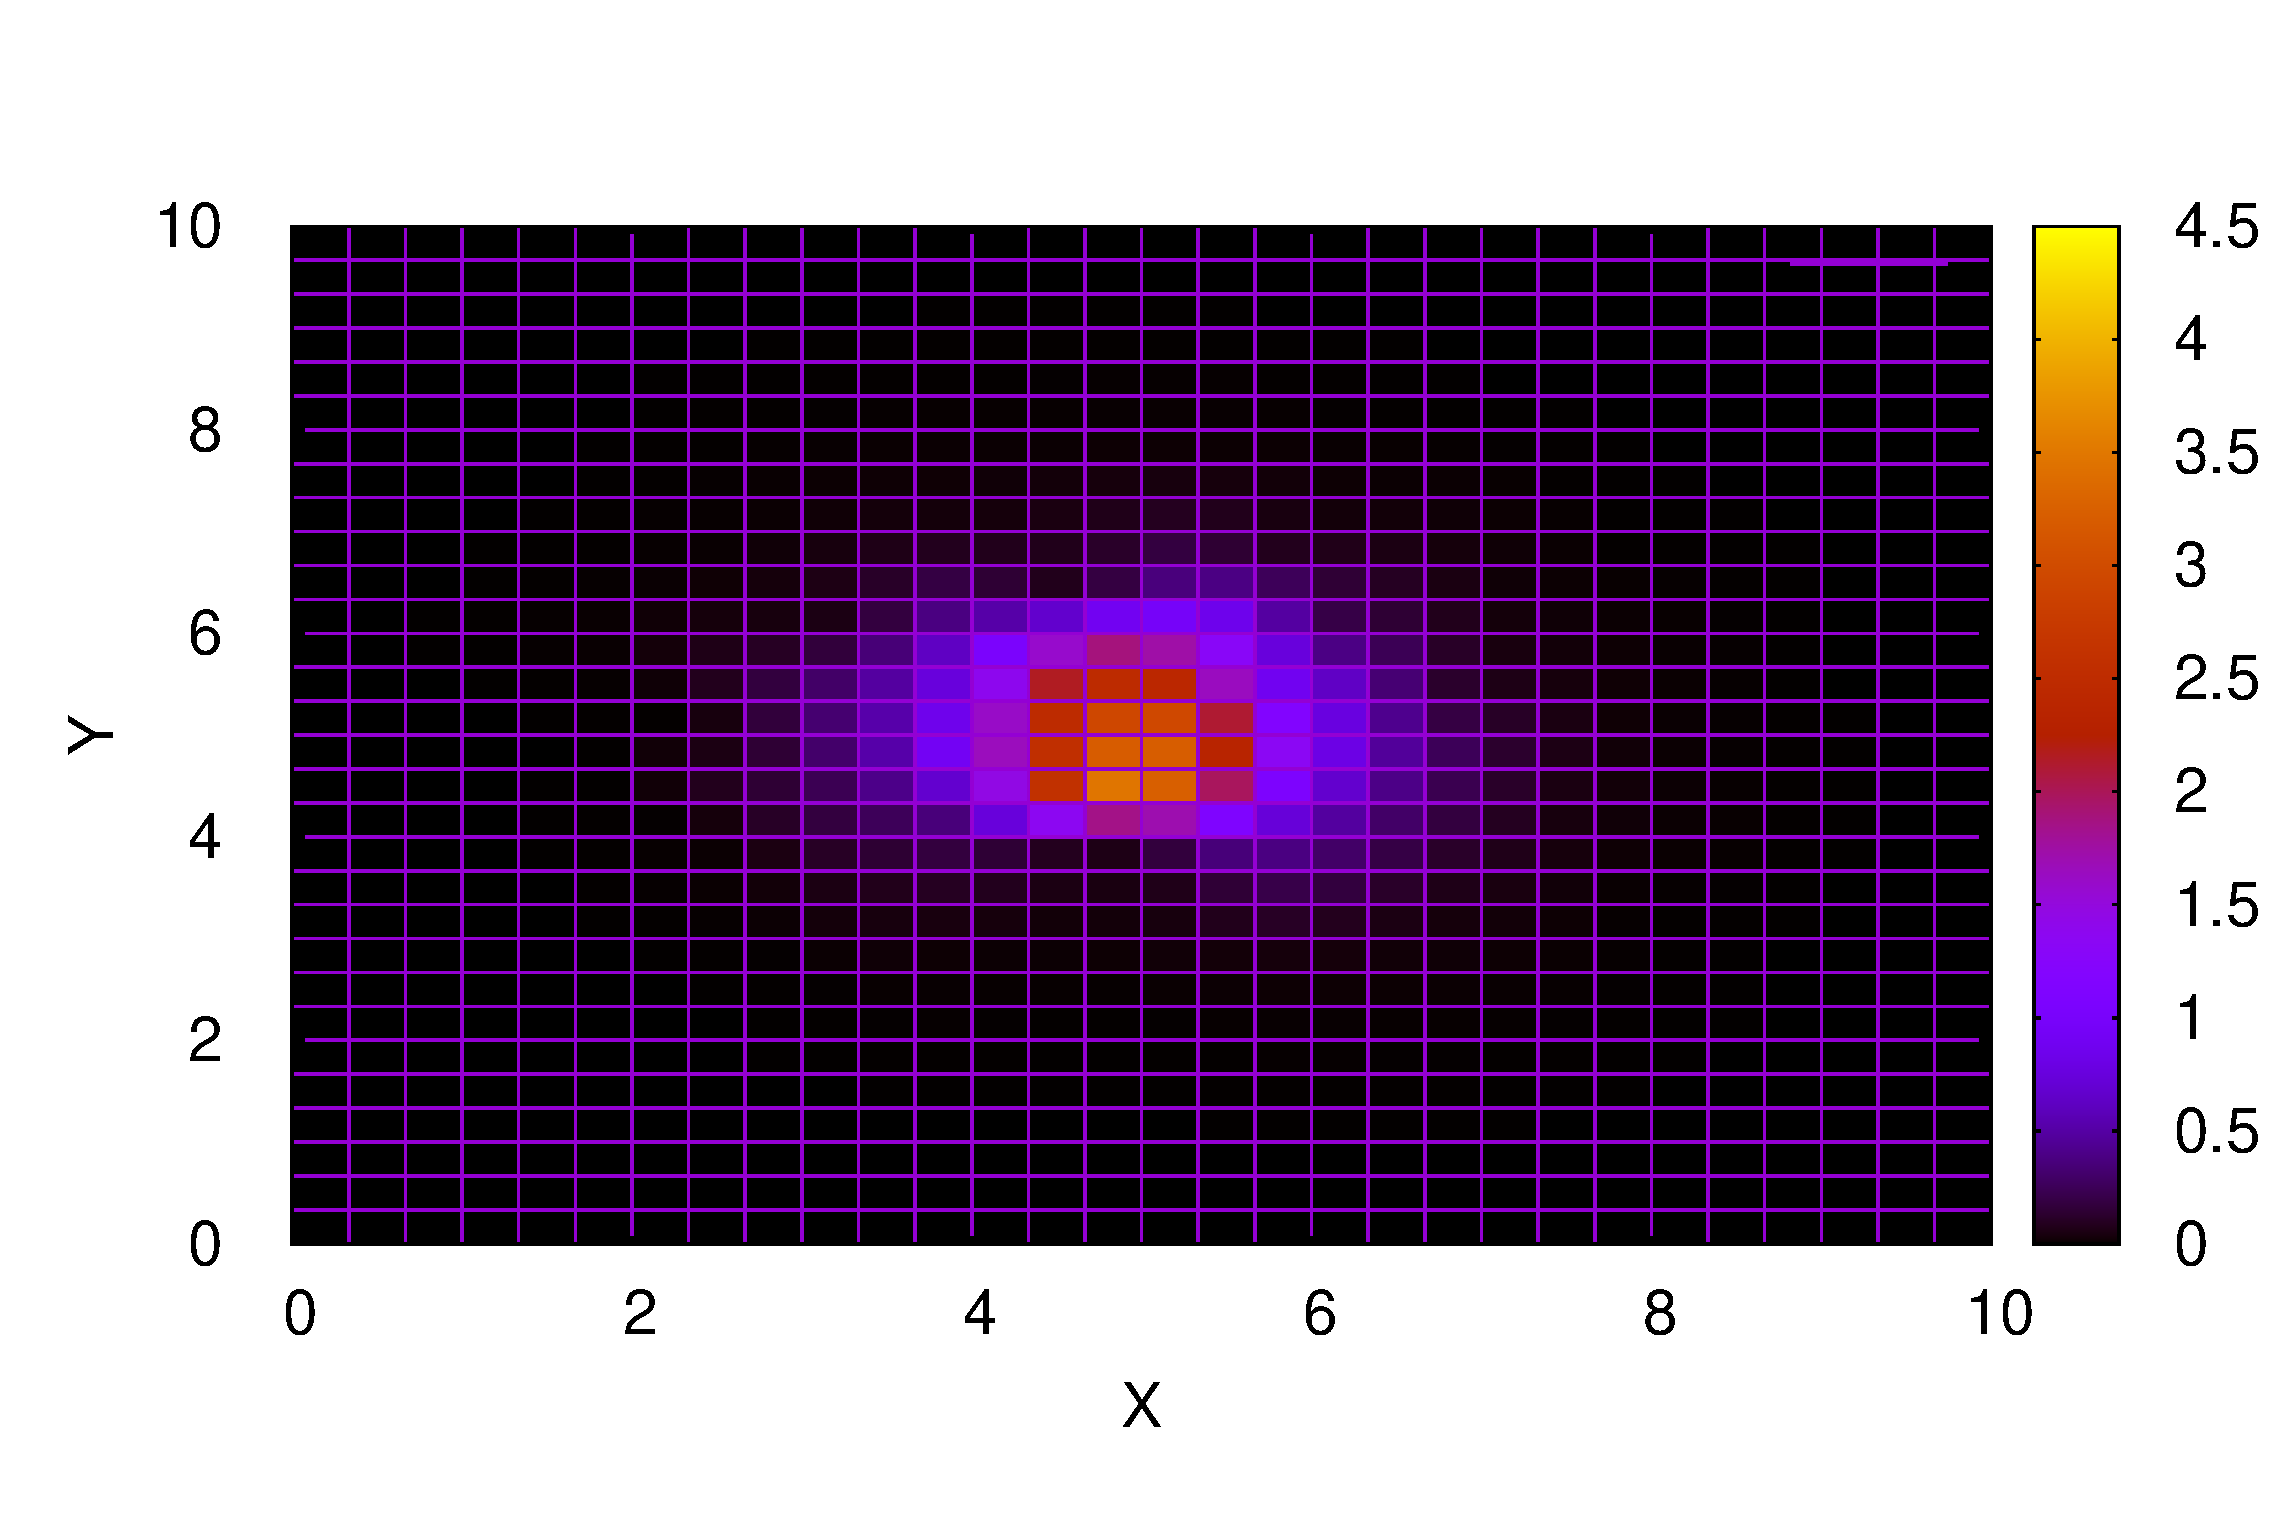
\includegraphics[width=\textwidth]{2DRandomDfig/05_map}
		\caption{the heat distribution map after 5 timesteps for the 2D heat problem}
		\label{fig:2d-randomD-5dt-map}
     \end{subfigure}
     \hfill
	\centering
     \begin{subfigure}[b]{0.45\textwidth}
         \centering
         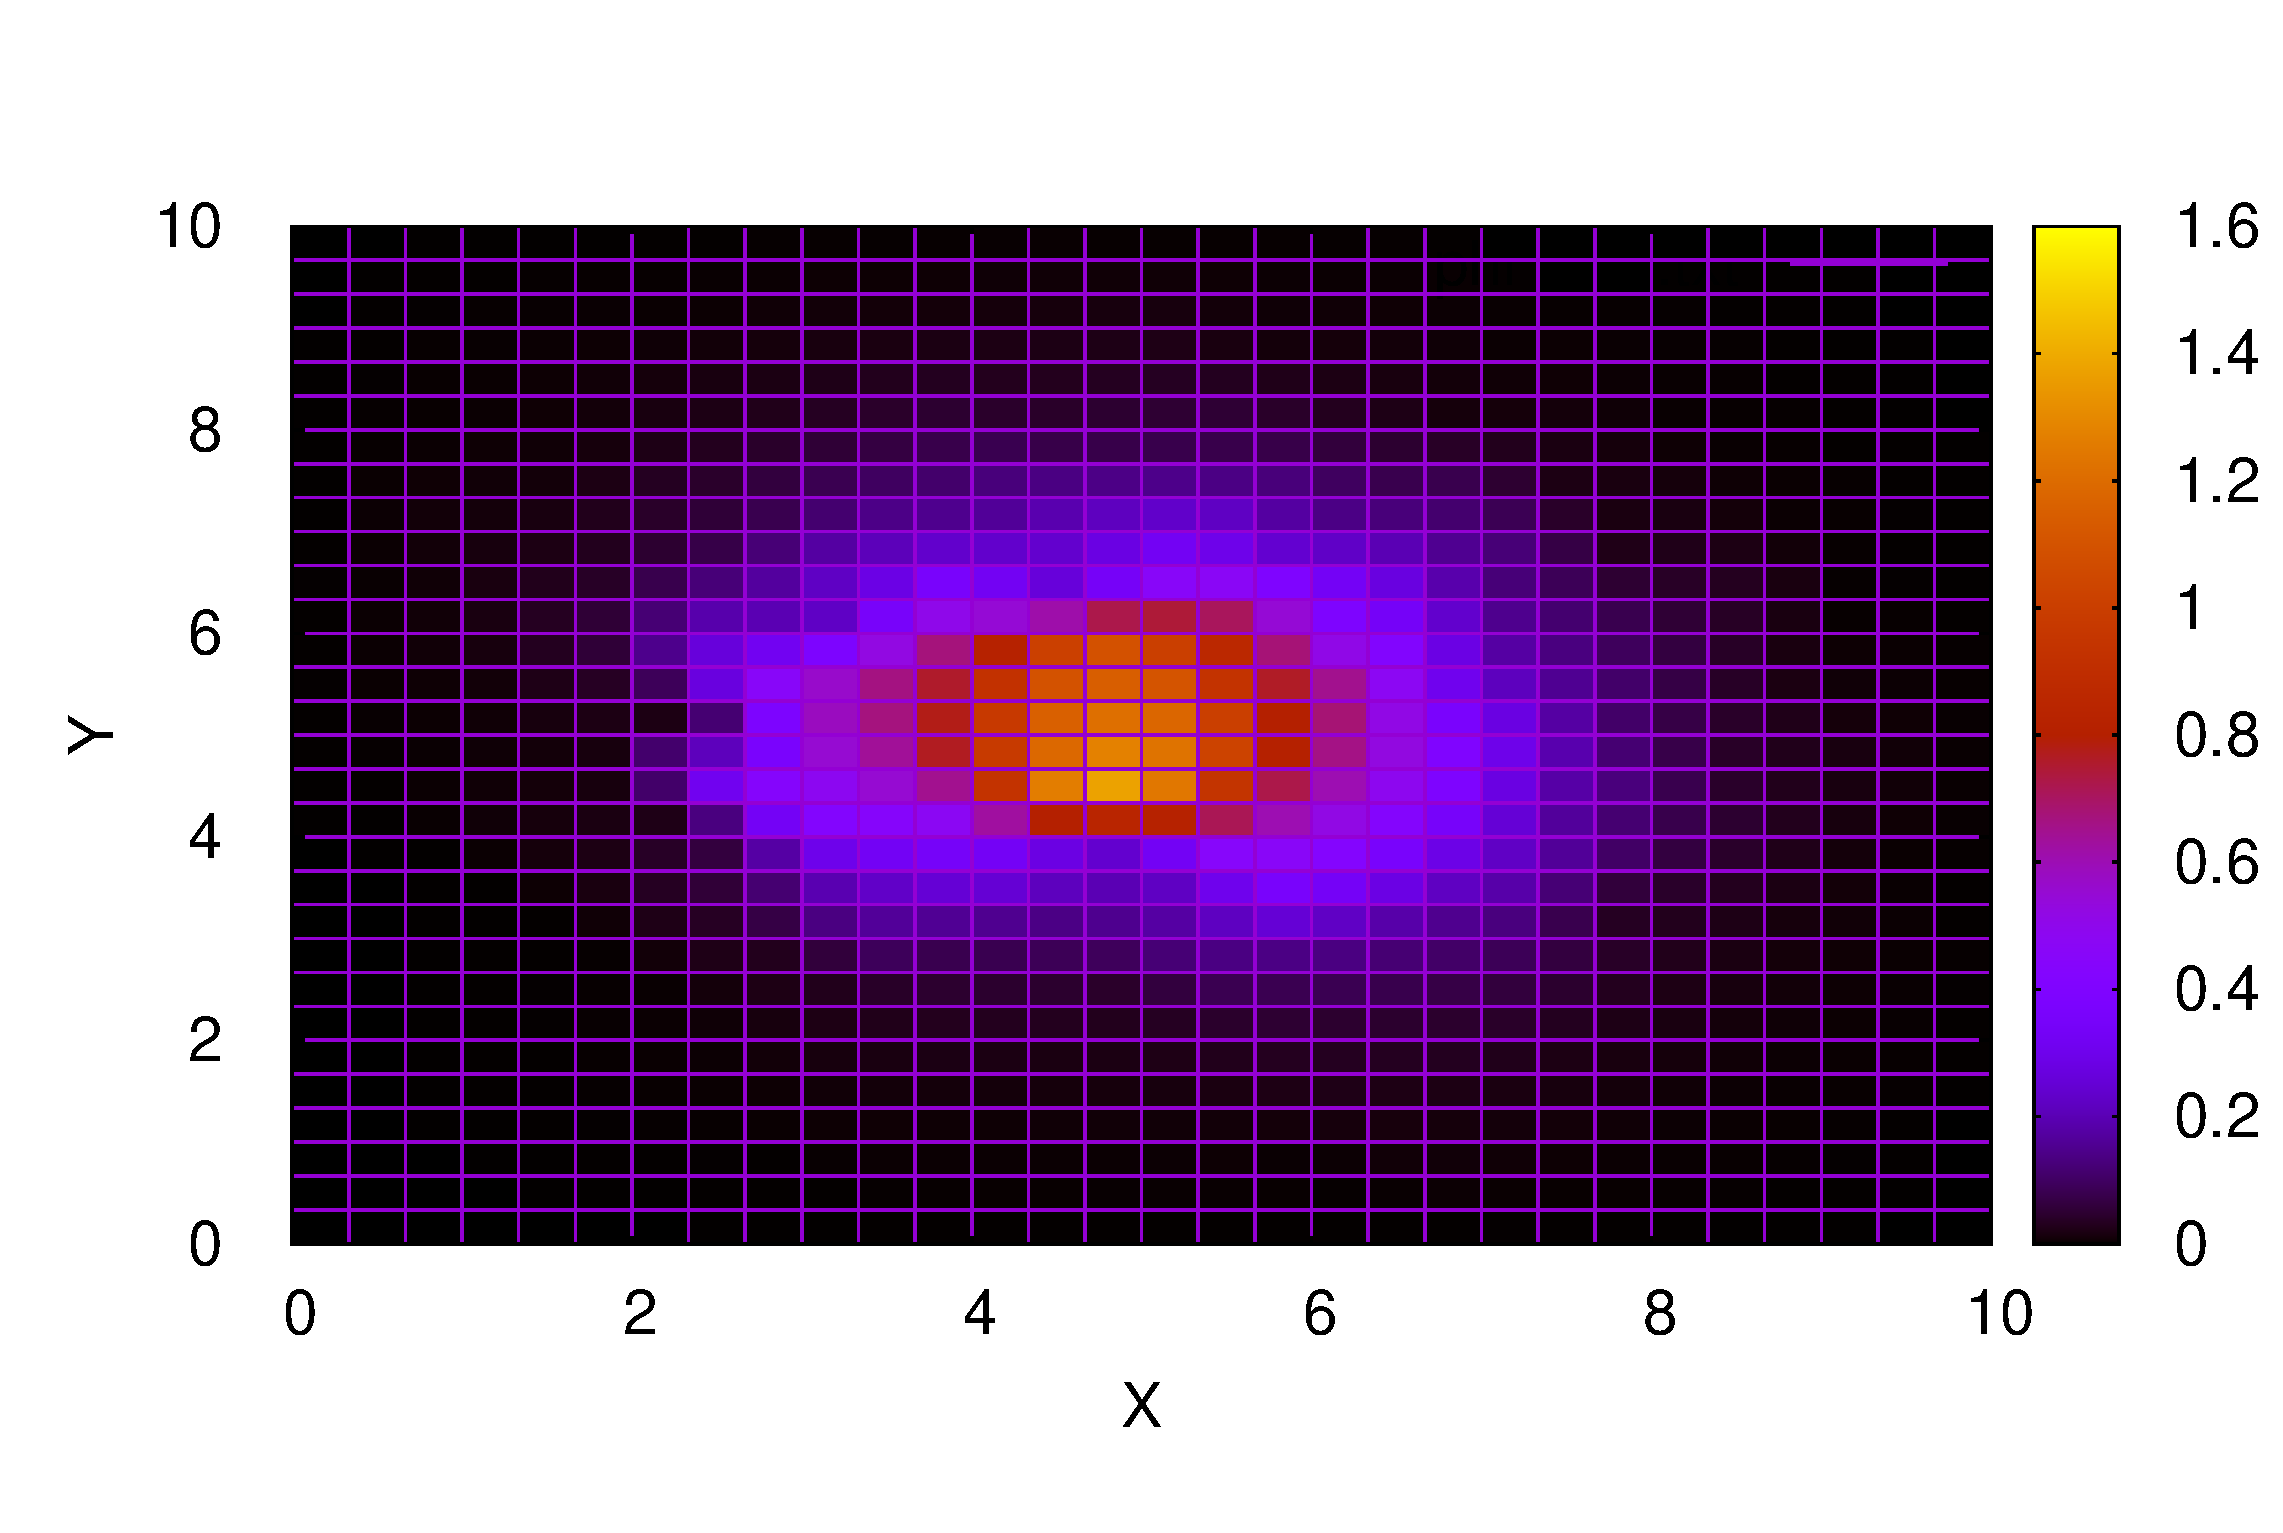
\includegraphics[width=\textwidth]{2DRandomDfig/15_map}
		\caption{the heat distribution map after 15 timesteps for the 2D heat problem}
		\label{fig:2d-randomD-15dt-map}
     \end{subfigure}
     \hfill     
          \begin{subfigure}[b]{0.45\textwidth}
         \centering
         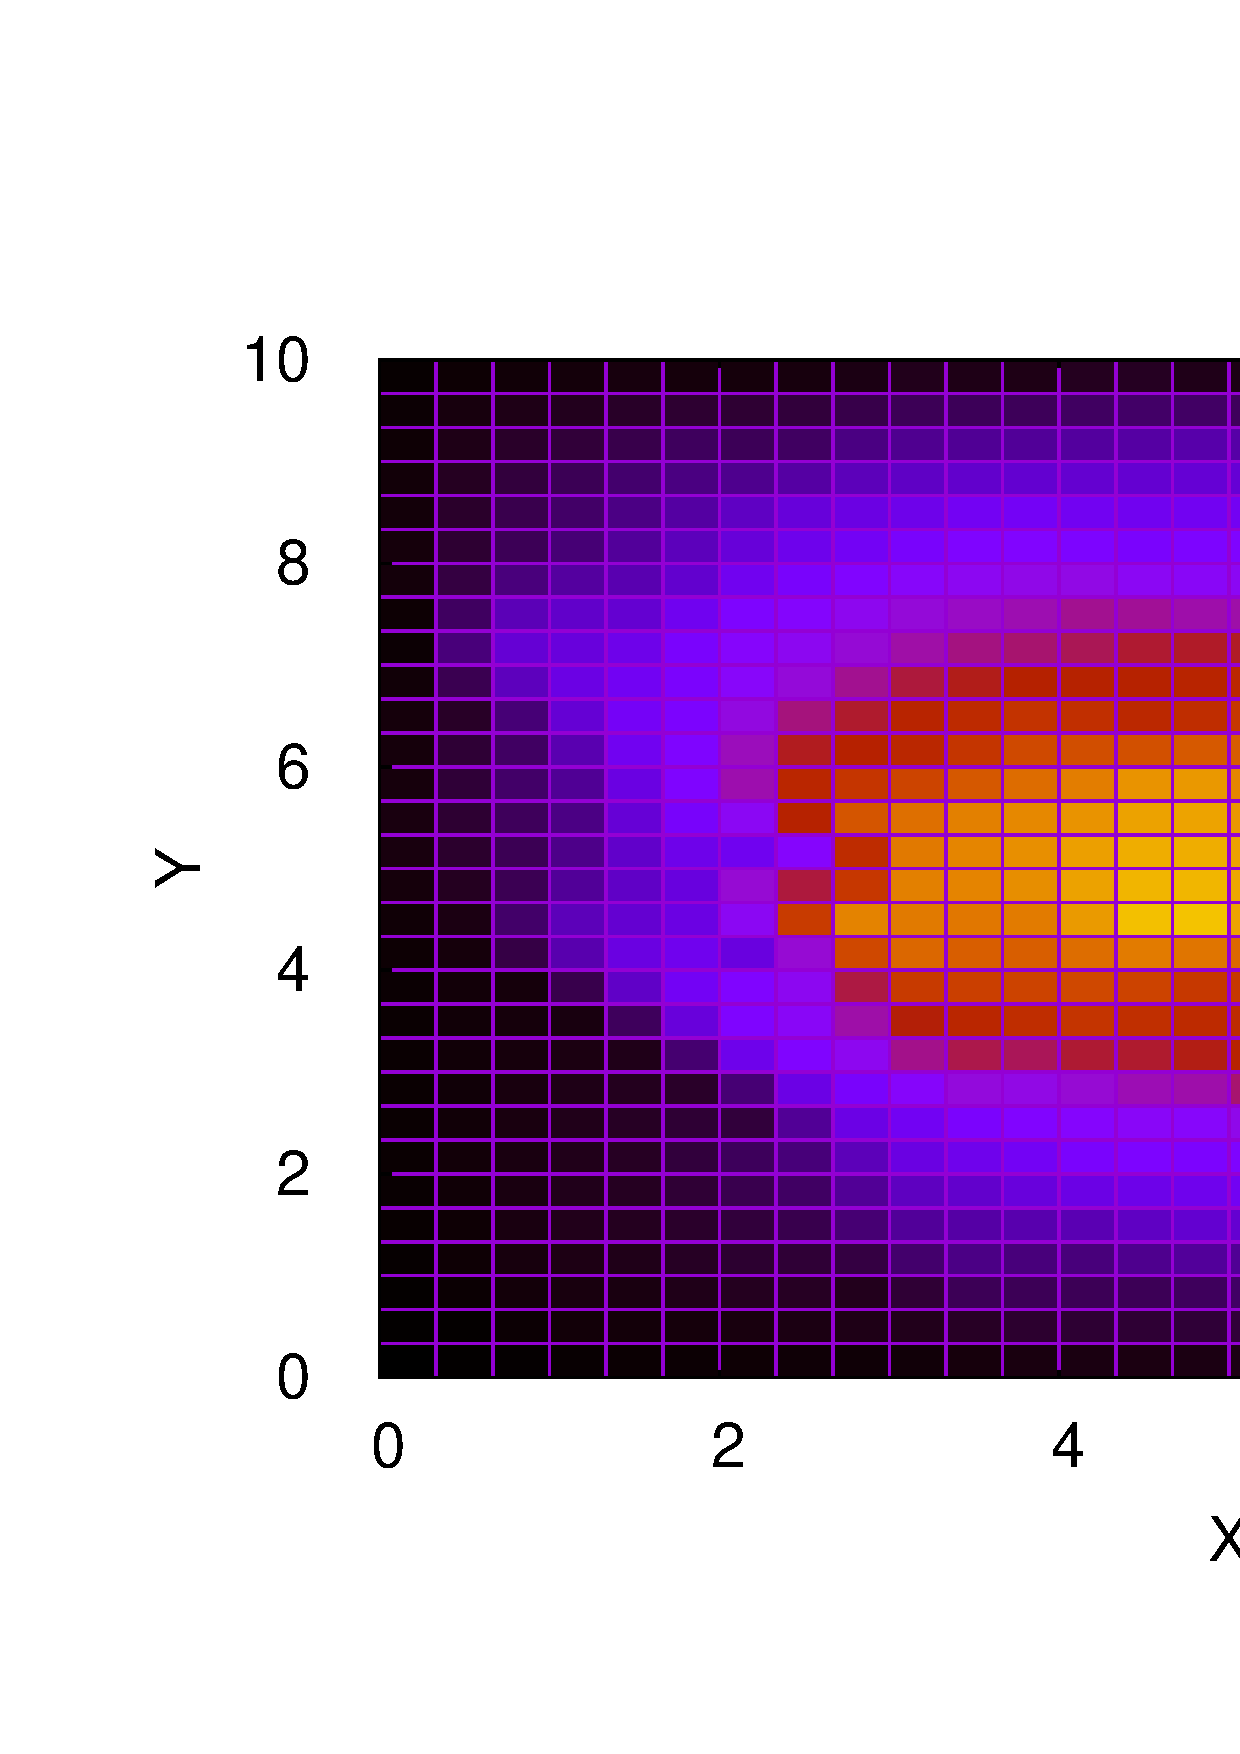
\includegraphics[width=\textwidth]{2DRandomDfig/45_map}
		\caption{the heat distribution map after 45 timesteps for the 2D heat problem}
		\label{fig:2d-randomD-45dt-map}
     \end{subfigure}
     \hfill     
        \caption{solving two-dimensional heat equation using CG method.}
        \label{fig:2d-CG-randomD}
\end{figure}

In contrast with the case of the constant diffusion coefficient, because of those random points which will not diffuse ($D(\vec{r}^{*})=0$), here the distribution of $\phi$ is not symmetric.

%stv
insert the plots for simple 2d and then the assignment here
